%%-----------------------------------------------------------------------------
%%
%%                                   Sean Mauch
%%                       California Institute of Technology
%%                          (a) 2000 No Rights Reserved
%%
%%-----------------------------------------------------------------------------

\flushbottom



%%============================================================================
%%============================================================================
\chapter{Cauchy's Integral Formula}







If I were founding a university I would begin with a smoking room; 
next a dormitory; and then a decent reading room and a library. 
After that, if I still had more money that I couldn't use, 
I would hire a professor and get some text books.

\begin{flushright}
  - Stephen Leacock
\end{flushright}










%%=============================================================================
\section{Cauchy's Integral Formula}



%% CONTINUE: compact?
\begin{Result}
  \label{cauchy}
  \textbf{Cauchy's Integral Formula.}
  If $f(\zeta)$ is analytic in a compact, closed, connected domain $D$ 
  and $z$ is a point in the interior of $D$ then
  \begin{equation}
    \label{eqn cauchy's integral formula}
    f(z) = \frac{1}{\imath 2 \pi} \oint_{\partial D} \frac{ f(\zeta) }{ \zeta - z } \,\dd \zeta
    = \frac{1}{\imath 2 \pi} \sum_k \oint_{C_k} \frac{ f(\zeta) }{ \zeta - z } \,\dd \zeta.
  \end{equation}
  Here the set of contours $\{ C_k \}$ make up the positively oriented boundary
  $\partial D$ of the domain $D$.  More generally, we have
  \begin{equation}
    \label{eqn cauchy's general integral formula}
    f^{(n)}(z) = \frac{n!}{\imath 2 \pi} \oint_{\partial D} \frac{ f(\zeta) }{ (\zeta - z)^{n+1} } \,\dd \zeta
    = \frac{n!}{\imath 2 \pi} \sum_k \oint_{C_k} \frac{ f(\zeta) }{ (\zeta - z)^{n+1} } \,\dd \zeta.
  \end{equation}
\end{Result}


Cauchy's Formula shows that the value of $f(z)$ and all its derivatives
in a domain are determined by the value of $f(z)$ on the boundary of 
the domain.
Consider the first formula of the result, Equation~
\ref{eqn cauchy's integral formula}.
We deform the contour to a circle of radius $\delta$ about the point $\zeta = z$.
%% CONTINUE figure
\begin{align*}
  \oint_C \frac{ f(\zeta) }{ \zeta - z } \,\dd \zeta
  &= \oint_{C_\delta} \frac{ f(\zeta) }{ \zeta - z } \,\dd \zeta 
  \\
  &= \oint_{C_\delta} \frac{ f(z) }{ \zeta - z } \,\dd \zeta
  + \oint_{C_\delta} \frac{ f(\zeta) - f(z) }{ \zeta - z } \,\dd \zeta
\end{align*}
We use the result of Example~\ref{ex_int1za} to evaluate the first integral.
\[
\oint_C \frac{ f(\zeta) }{ \zeta - z } \,\dd \zeta
= \imath 2 \pi f(z)
+ \oint_{C_\delta} \frac{ f(\zeta) - f(z) }{ \zeta - z } \,\dd \zeta 
\]
The remaining integral along $C_\delta$ vanishes as $\delta \to 0$
because $f(\zeta)$ is continuous.
We demonstrate this with the maximum modulus integral bound.  The length
of the path of integration is $2 \pi \delta$.
\begin{align*}
  \lim_{\delta \to 0}
  \left| \oint_{C_\delta} \frac{ f(\zeta) - f(z) }{ \zeta - z } \,\dd \zeta \right|
  &\leq \lim_{\delta \to 0} \left( (2 \pi \delta) \frac{1}{\delta} \max_{|\zeta - z| = \delta} |f(\zeta) - f(z)| \right) 
  \\
  &\leq \lim_{\delta \to 0} \left( 2 \pi \max_{|\zeta - z| = \delta} |f(\zeta) - f(z)| \right) 
  \\
  &= 0
\end{align*}
This gives us the desired result.
\[
f(z) = \frac{1}{\imath 2 \pi} \oint_C \frac{ f(\zeta) }{ \zeta - z } \,\dd \zeta
\]

We derive the second formula, Equation~
\ref{eqn cauchy's general integral formula},
from the first by differentiating with 
respect to $z$.  Note that the integral converges uniformly for $z$ in
any closed subset of the interior of $C$.  Thus we can differentiate
with respect to $z$ and interchange the order of differentiation 
and integration.  
\begin{align*}
  f^{(n)}(z) &= \frac{1}{\imath 2 \pi} \frac{\dd^n}{\dd z^n} 
  \oint_C \frac{ f(\zeta) }{ \zeta - z } \,\dd \zeta 
  \\
  &= \frac{1}{\imath 2 \pi} \oint_C \frac{\dd^n}{\dd z^n} \frac{ f(\zeta) }{ \zeta - z } \,\dd \zeta 
  \\
  &= \frac{n!}{\imath 2 \pi} \oint_C \frac{ f(\zeta) }{ (\zeta - z)^{n+1} } \,\dd \zeta
\end{align*}




%% CONTINUE: prove for multiply-connected domains as an exercise.
%%           Use Cauchy's theorem.




\begin{Example}
  Consider the following integrals where $C$ is the positive contour on the
  unit circle.
  For the third integral, the point $z = -1$ is removed from the contour.
  \begin{enumerate}
  \item
    $ \displaystyle \oint_C \sin \left( \cos \left( z^5 \right) \right)\,\dd z$
  \item
    $ \displaystyle \oint_C \frac{1}{(z - 3) (3 z - 1)}\,\dd z$
  \item
    $ \displaystyle \int_C \sqrt{z}\,\dd z$
  \end{enumerate}


  \begin{enumerate}
  \item
    Since $\sin \left( \cos \left( z^5 \right) \right)$ 
    is an analytic function inside the unit circle,
    \[
    \oint_C \sin \left( \cos \left( z^5 \right) \right)\,\dd z = 0
    \]
    %%
    %%
  \item
    $\frac{1}{(z - 3) (3 z - 1)}$ has singularities at $z = 3$ and $z = 1/3$.
    Since $z = 3$ is outside the contour, only the singularity at $z = 1/3$
    will contribute to the value of the integral.  We will evaluate this
    integral using the Cauchy integral formula.
    \[
    \oint_C \frac{1}{(z - 3) (3 z - 1)}\,\dd z  
    = \imath 2 \pi \left( \frac{1}{(1/3 - 3) 3} \right)
    = - \frac{\imath \pi}{4}
    \]
    %%
    %%
  \item
    Since the curve is not closed, we cannot apply the Cauchy integral
    formula.  Note that $\sqrt{z}$ is single-valued and analytic in
    the complex plane with a branch cut on the negative real axis.
    Thus we use the Fundamental Theorem of Calculus.
    \begin{align*}
      \int_C \sqrt{z}\,\dd z
      &= \left[ \frac{2}{3} \sqrt{z^3} \right]_{\e^{-\imath \pi}}^{\e^{\imath \pi}} 
      \\
      &= \frac{2}{3} \left( \e^{\imath 3 \pi / 2} - \e^{-\imath 3 \pi / 2} \right) 
      \\
      &= \frac{2}{3} (-\imath - \imath) 
      \\
      &= - \imath \frac{4}{3}
    \end{align*}
  \end{enumerate}
\end{Example}










\paragraph{Cauchy's Inequality.}
Suppose the $f(\zeta)$ is analytic in the closed disk $|\zeta - z| \leq r$.
By Cauchy's integral formula, 
\[
f^{(n)}(z) = \frac{n!}{\imath 2 \pi} \oint_C \frac{ f(\zeta) }{ (\zeta - z)^{n+1} }\,\dd \zeta,
\]
where $C$ is the circle of radius $r$ centered about the point $z$.   We use
this to obtain an upper bound on the modulus of $f^{(n)}(z)$.
\begin{align*}
  \left| f^{(n)}(z) \right|
  &= \frac{n!}{2 \pi} \left| \oint_C \frac{ f(\zeta) }{ (\zeta - z)^{n+1} }\,\dd \zeta \right| 
  \\
  &\leq \frac{n!}{2 \pi} 2 \pi r \max_{|\zeta - z| = r} \left| 
    \frac{ f(\zeta) }{ (\zeta - z)^{n+1} } \right| 
  \\
  &= \frac{ n! }{ r^n } \max_{|\zeta - z| = r} \left| f(\zeta) \right| 
\end{align*}



\begin{Result}
  \label{cauchy_inequality}
  \index{Cauchy's inequality}
  \textbf{Cauchy's Inequality.}
  If $f(\zeta)$ is analytic in $|\zeta - z| \leq r$ then
  \[
  \left| f^{(n)}(z) \right| \leq \frac{ n! M }{ r^n }
  \]
  where $|f(\zeta)| \leq M$ for all $|\zeta - z| = r$.
\end{Result}






\paragraph{Liouville's Theorem.}
Consider a function $f(z)$ that is analytic and bounded, ($|f(z)| \leq M$), 
in the complex plane.  From Cauchy's inequality, 
\[
|f'(z)| \leq \frac{M}{r}
\]
for any positive $r$.  By taking $r \to \infty$, we see that $f'(z)$ is
identically zero for all $z$.  Thus $f(z)$ is a constant.



\begin{Result}
  \label{liouvilles_theorem}
  \index{Liouville's theorem}
  \textbf{Liouville's Theorem.}
  If $f(z)$ is analytic and $|f(z)|$ is bounded in the complex plane then 
  $f(z)$ is a constant.
\end{Result}








\paragraph{The Fundamental Theorem of Algebra.}
We will prove that every polynomial of degree $n \geq 1$ has exactly $n$
roots, counting multiplicities.  First we demonstrate that each such
polynomial has at least one root.  Suppose that an $n^{\mathrm{th}}$ degree
polynomial $p(z)$ has no roots.  Let the lower bound on the modulus of 
$p(z)$ be $0 < m \leq |p(z)|$.  The function $f(z) = 1 / p(z)$ is
analytic, ($f'(z) = p'(z) / p^2(z)$), and bounded, ($|f(z)| \leq 1/m$), 
in the extended complex plane.   Using Liouville's theorem we conclude
that $f(z)$ and hence $p(z)$ are constants, which yields a contradiction.
Therefore every such polynomial $p(z)$ must have at least one root.

Now we show that we can factor the root out of the polynomial.
Let
\[
p(z) = \sum_{k = 0}^n p_k z^k.
\]
We note that
\[
\left( z^n - c^n \right) = (z - c) \sum_{k = 0}^{n-1} c^{n-1-k} z^k.
\]
Suppose that the $n^{\mathrm{th}}$ degree polynomial $p(z)$ has a root at $z = c$.
\begin{align*}
  p(z)    
  &= p(z) - p(c) 
  \\
  &= \sum_{k = 0}^n p_k z^k - \sum_{k = 0}^n p_k c^k 
  \\
  &= \sum_{k = 0}^n p_k \left( z^k - c^k \right)
  \\
  &= \sum_{k = 0}^n p_k (z - c) \sum_{j = 0}^{k-1} c^{k-1-j} z^j 
  \\
  &= (z - c) q(z)
\end{align*}
Here $q(z)$ is a polynomial of degree $n - 1$.  By induction, we see that
$p(z)$ has exactly $n$ roots.






\begin{Result}
  \label{fundamental_theorem_of_algebra}
  \index{fundamental theorem of algebra}
  \textbf{Fundamental Theorem of Algebra.}
  Every polynomial of degree $n \geq 1$ has exactly $n$ roots, counting 
  multiplicities.
\end{Result}








\paragraph{Gauss' Mean Value Theorem.}
Let $f(\zeta)$ be analytic in $|\zeta - z| \leq r$.  By Cauchy's integral
formula,
\[
f(z) = \frac{1}{\imath 2 \pi} \oint_C \frac{ f(\zeta) }{ \zeta - z } \,\dd \zeta,
\]
where $C$ is the circle $|\zeta - z| = r$.  We parameterize the contour
with $\zeta = z + r \e^{\imath \theta}$.
\[
f(z) = \frac{1}{\imath 2 \pi} 
\int_0^{2 \pi} \frac{ f(z + r \e^{\imath \theta}) }{ r \e^{\imath \theta} } \imath r \e^{\imath \theta}\,\dd \theta
\]
Writing this in the form,
\[
f(z) = \frac{1}{2 \pi r} \int_0^{2 \pi} f(z + r \e^{\imath \theta}) r\,\dd \theta,
\]
we see that $f(z)$ is the average value of $f(\zeta)$ on the circle of radius
$r$ about the point $z$.




\begin{Result}
  \label{gauss_average_value_theorem}
  \index{average value theorem}
  \textbf{Gauss' Average Value Theorem.}
  If $f(\zeta)$ is analytic in $|\zeta - z| \leq r$ then
  \[
  f(z) = \frac{1}{2 \pi} \int_0^{2 \pi} f(z + r \e^{\imath \theta})\,\dd \theta.
  \]
  That is, $f(z)$ is equal to its average value on a circle of radius $r$
  about the point $z$.
\end{Result}







\paragraph{Extremum Modulus Theorem.}
Let $f(z)$ be analytic in closed, connected domain, $D$.  The extreme values
of the modulus of the function must occur on the boundary.  If $|f(z)|$ has
an interior extrema, then the function is a constant.  We will show this
with proof by contradiction.  Assume that $|f(z)|$ has an interior maxima at
the point $z = c$.  This means that there exists an neighborhood of the
point $z = c$ for which $|f(z)| \leq |f(c)|$.  Choose an $\epsilon$ so that
the set $|z - c| \leq \epsilon$ lies inside this neighborhood.  First we 
use Gauss' mean value theorem.
\[
f(c) = \frac{1}{2 \pi} \int_0^{2 \pi} f \left(c + \epsilon \e^{\imath \theta} \right)\,\dd \theta
\]
We get an upper bound on $|f(c)|$ with the maximum modulus integral bound.
\[
|f(c)| \leq \frac{1}{2 \pi} \int_0^{2 \pi} \left| 
  f \left(c + \epsilon \e^{\imath \theta} \right) \right| \,\dd \theta
\]
Since $z = c$ is a maxima of $|f(z)|$ we can get a lower bound on $|f(c)|$.
\[
|f(c)| \geq \frac{1}{2 \pi} \int_0^{2 \pi} \left| 
  f \left(c + \epsilon \e^{\imath \theta} \right) \right| \,\dd \theta
\]
If $|f(z)| < |f(c)|$ for any point on $|z - c| = \epsilon$, 
then the continuity of $f(z)$ 
implies that $|f(z)| < |f(c)|$ in a neighborhood of that point which would
make the value of the integral of $|f(z)|$ strictly less than $|f(c)|$.  Thus 
we conclude that $|f(z)| = |f(c)|$ for all $|z - c| = \epsilon$.  Since we
can repeat the above procedure for any circle of radius smaller than 
$\epsilon$, $|f(z)| = |f(c)|$ for all $|z - c| \leq \epsilon$, i.e. all the
points in the disk of radius $\epsilon$ about $z = c$ are also maxima.
By recursively repeating this procedure points in this disk, we see that
$|f(z)| = |f(c)|$ for all $z \in D$.    This implies that $f(z)$ is a constant
in the domain.  By reversing the inequalities in the above method we 
see that the minimum modulus of $f(z)$ must also occur on the boundary.





\begin{Result}
  \label{extremum_modulus_theorem}
  \index{extremum modulus theorem}
  \index{maximum modulus theorem}
  \index{minimum modulus theorem}
  \textbf{Extremum Modulus Theorem.}
  Let $f(z)$ be analytic in a closed, connected domain, $D$.  The
  extreme values of the modulus of the function must occur on the
  boundary.  If $|f(z)|$ has an interior extrema, then the function
  is a constant.
\end{Result}













%%=============================================================================
\section{The Argument Theorem}
\index{argument theorem}



\begin{Result}
  \label{res_argument_theorem}
  \textbf{The Argument Theorem.}
  Let $f(z)$ be analytic inside and on $C$ except for isolated poles inside
  the contour.  Let $f(z)$ be nonzero on $C$.
  \[
  \frac{1}{\imath 2 \pi} \int_C \frac{f'(z)}{f(z)}\,\dd z = N - P
  \]
  Here $N$ is the number of zeros and $P$ the number of poles,
  counting multiplicities, of $f(z)$ inside $C$.
\end{Result}


First we will simplify the problem and consider a function $f(z)$ that has 
one zero or one pole.
Let $f(z)$ be analytic and nonzero inside and on $A$ except for a zero of 
order $n$ at $z = a$.  Then we can write $f(z) = (z-a)^n g(z)$ where $g(z)$ is 
analytic and nonzero inside and on $A$.  The integral of $\frac{f'(z)}{f(z)}$
along $A$ is
\begin{align*}
  \frac{1}{\imath 2 \pi} \int_A \frac{f'(z)}{f(z)}\,\dd z
  &= \frac{1}{\imath 2 \pi} \int_A \frac{\dd}{\dd z} \left( \log(f(z)) \right)\,\dd z
  \\
  &= \frac{1}{\imath 2 \pi} \int_A \frac{\dd}{\dd z} \left( \log((z - a)^n) + 
    \log(g(z)) \right)\,\dd z 
  \\
  &= \frac{1}{\imath 2 \pi} \int_A \frac{\dd}{\dd z} \left( \log((z - a)^n) 
  \right)\,\dd z 
  \\
  &= \frac{1}{\imath 2 \pi} \int_A \frac{n}{z - a} \,\dd z 
  \\
  &= n
\end{align*}

Now let $f(z)$ be analytic and nonzero inside and on $B$ except for a pole of 
order $p$ at $z = b$.  Then we can write $f(z) = \frac{g(z)}{(z - b)^p}$ 
where $g(z)$ is analytic and nonzero inside and on $B$.  The integral of 
$\frac{f'(z)}{f(z)}$ along $B$ is
\begin{align*}
  \frac{1}{\imath 2 \pi} \int_B \frac{f'(z)}{f(z)}\,\dd z
  &= \frac{1}{\imath 2 \pi} \int_B \frac{\dd}{\dd z} \left( \log(f(z)) \right)
  \,\dd z 
  \\
  &= \frac{1}{\imath 2 \pi} \int_B \frac{\dd}{\dd z} \left( \log((z - b)^{-p}) + 
    \log(g(z)) \right)\,\dd z 
  \\
  &= \frac{1}{\imath 2 \pi} \int_B \frac{\dd}{\dd z} \left( \log((z - b)^{-p}) + 
  \right)\,\dd z 
  \\
  &= \frac{1}{\imath 2 \pi} \int_B \frac{- p}{z - b}\,\dd z 
  \\
  &= - p
\end{align*}



Now consider a function $f(z)$ that is analytic inside an on the contour
$C$ except for isolated poles at the points $b_1, \ldots, b_p$.  Let
$f(z)$ be nonzero except at the isolated points $a_1, \ldots, a_n$.
Let the contours $A_k$, $k=1,\ldots,n$, be simple, positive contours which 
contain the zero at $a_k$ but no other poles or zeros of $f(z)$.  
Likewise, let the contours $B_k$, $k=1,\ldots,p$ be simple, positive contours 
which contain the pole at $b_k$ but no other poles of zeros of $f(z)$.
(See Figure~\ref{ci_argth}.)  By deforming the contour we obtain
\[
\int_C \frac{f'(z)}{f(z)} \,\dd z
= \sum_{j=1}^n \int_{A_j} \frac{f'(z)}{f(z)} \,\dd z
+ \sum_{k=1}^p \int_{B_j} \frac{f'(z)}{f(z)} \,\dd z.
\]
From this we obtain Result~\ref{res_argument_theorem}. 

\begin{figure}[htb!]
  \begin{center}
    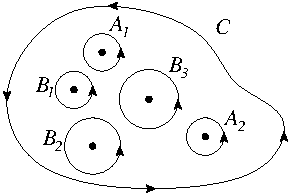
\includegraphics[width=0.3\textwidth]{fcv/cauchy/ci_argth}
  \end{center}
  \caption{Deforming the contour.}
  \label{ci_argth}
\end{figure}


%%We can generalize the argument theorem.  (See Exercise~\ref{ci_gen_arg}.)

%%\begin{Result}
%%\textbf{The Argument Theorem.}
%%Let $g(z)$ be analytic inside and on $C$.
%%Let $f(z)$ be analytic and nonzero inside and on $C$ except for 
%%zeros at $a_1,\ldots,a_n$ and isolated poles at $b_1,\ldots,b_p$ inside
%%the contour.  Let $f(z)$ be nonzero on $C$.
%%\[
%%\frac{1}{\imath 2 \pi} \int_C \frac{f'(z)}{f(z)}\,\dd z 
%%= \sum_{j=1}^n g(a_j)
%%CONTINUE
%%\]
%%Here $N$ is the number of zeros and $P$ the number of poles,
%%counting multiplicities, of $f(z)$ inside $C$.
%%\end{Result}






%%=============================================================================
\section{Rouche's Theorem}
\index{Rouche's theorem}



\begin{Result}
  \label{rouches_theorem}
  \textbf{Rouche's Theorem.}
  Let $f(z)$ and $g(z)$ be analytic inside and on a simple, closed contour
  $C$.   If $|f(z)| > |g(z)|$ on $C$ then $f(z)$ and $f(z) + g(z)$ have
  the same number of zeros inside $C$ and no zeros on $C$.
\end{Result}


First note that since $|f(z)| > |g(z)|$ on $C$, $f(z)$ is nonzero on $C$.
The inequality implies that $|f(z) + g(z)| > 0$ on $C$ so $f(z) + g(z)$
has no zeros on $C$.  We well count the number of zeros of $f(z)$ and 
$g(z)$ using the Argument Theorem, (Result~\ref{res_argument_theorem}). 
The number of zeros $N$ of $f(z)$ inside the contour is 
\[
N = \frac{1}{\imath 2 \pi} \oint_C \frac{ f'(z) }{ f(z) } \,\dd z.
\]
Now consider the number of zeros $M$ of $f(z) + g(z)$.  We introduce the
function $h(z) = g(z) / f(z)$.
\begin{align*}
  M       
  &= \frac{1}{\imath 2 \pi} \oint_C \frac{ f'(z) + g'(z) }{ f(z) + g(z) }\,\dd z 
  \\
  &= \frac{1}{\imath 2 \pi} \oint_C \frac{ f'(z) + f'(z) h(z) + f(z) h'(z) }
  { f(z) + f(z) h(z) }\,\dd z 
  \\
  &= \frac{1}{\imath 2 \pi} \oint_C \frac{ f'(z) }{ f(z) } \,\dd z
  + \frac{1}{\imath 2 \pi} \oint_C \frac{ h'(z) }{ 1 + h(z) } \,\dd z 
  \\
  &= N + \frac{1}{\imath 2 \pi} \left[ \log(1 + h(z)) \right]_C 
  \\
  &= N
\end{align*}
(Note that since $|h(z)| < 1$ on $C$, $\Re(1 + h(z)) > 0$ on $C$
and the value of $\log(1 + h(z))$ does not not change in traversing the
contour.)
This demonstrates that $f(z)$ and $f(z) + g(z)$ have the same number of 
zeros inside $C$ and proves the result.















\raggedbottom
%%=============================================================================
\exercises{
\pagebreak
\flushbottom
\section{Exercises}







%%
\begin{Exercise}
  What is
  \[
  (\arg(\sin z))\big|_{C}
  \]
  where $C$ is the unit circle?
\end{Exercise}




%% Three integrals.
\begin{Exercise}
  Let $C$ be the circle of radius $2$ centered about the origin and oriented
  in the positive direction.  Evaluate the following integrals:
  \begin{enumerate}
  \item $\oint_C \frac{\sin z}{z^2 + 5}\,\dd z$
  \item $\oint_C \frac{z}{z^2 + 1}\,\dd z$
  \item $\oint_C \frac{z^2 + 1}{z}\,\dd z$
  \end{enumerate}
\end{Exercise}





%% f(z) is constant.
\begin{Exercise}
  Let $f(z)$ be analytic and bounded (i.e. $|f(z)| < M$) for $|z| > R$, but not
  necessarily analytic for $|z| \leq R$. 
  Let the points $\alpha$ and $\beta$ lie inside the circle $|z| = R$.
  Evaluate 
  \[
  \oint_C \frac{f(z)}{(z - \alpha) (z - \beta)}\,\dd z
  \]
  where $C$ is any closed contour outside $|z| = R$, containing the circle 
  $|z| = R$.
  [Hint: consider the circle at infinity]
  Now suppose that in addition $f(z)$ is analytic everywhere.
  Deduce that $f(\alpha) = f(\beta)$.
\end{Exercise}








%% $p(z) = z^6 - 5 z^2 + 10 = 0$ lie in the annulus $1 < |z| < 2$.
\begin{Exercise}
  Using Rouche's theorem show that all the roots of the equation
  $p(z) = z^6 - 5 z^2 + 10 = 0$ lie in the annulus $1 < |z| < 2$.
\end{Exercise}









%% \omega = \frac{1}{2 \pi \imath} \oint_C \frac{e^{zt}}{z^2(z^2 + a^2)} \dd z,
\begin{Exercise}
  Evaluate as a function of $t$
  \[
  \omega = \frac{1}{\imath 2 \pi} \oint_C \frac{\e^{z t}}{z^2 (z^2 + a^2)}\,\dd z,
  \]
  where $C$ is any positively oriented contour surrounding the circle 
  $|z| = a$.
\end{Exercise}




\begin{Exercise}
  Consider $C_1$, (the positively oriented circle $|z| = 4$), and $C_2$,
  (the positively oriented boundary of the square whose sides lie along the 
  lines $x = \pm 1$, $y = \pm 1$).  Explain why
  \[
  \int_{C_1} f(z) \,\dd z = \int_{C_2} f(z) \,\dd z
  \]
  for the functions
  \begin{enumerate}
  \item 
    $\displaystyle f(z) = \frac{1}{3 z^2 + 1}$
  \item 
    $\displaystyle f(z) = \frac{z}{1 - \e^z}$
  \end{enumerate}
\end{Exercise}









\begin{Exercise}
  Show that if $f(z)$ is of the form
  \[
  f(z) = \frac{\alpha_k}{z^k} + \frac{\alpha_{k-1}}{z^{k-1}} + \cdots +\frac{\alpha_1}{z} + g(z), \quad k \geq 1
  \]
  where $g$ is analytic inside and on $C$, (the positive circle $|z| = 1$), then
  \[
  \int_C f(z)\,\dd z = \imath 2 \pi \alpha_1.
  \]  
\end{Exercise}







\begin{Exercise}
  Show that if $f(z)$ is analytic within and on a simple closed contour $C$ and
  $z_0$ is not on $C$ then
  \[
  \int_C \frac{f'(z)}{z - z_0}\,\dd z = \int_C \frac{f(z)}{(z - z_0)^2}\,\dd z.
  \]
  Note that $z_0$ may be either inside or outside of $C$.
\end{Exercise}








\begin{Exercise}
  If $C$ is the positive circle $z = \e^{\imath \theta}$ show that for any real constant $a$,
  \[
  \int_C \frac{\e^{a z}}{z} \,\dd z = \imath 2 \pi
  \]
  and hence
  \[
  \int_0^\pi \e^{a \cos \theta} \cos(a \sin \theta)\,\dd \theta = \pi.
  \]
\end{Exercise}









\begin{Exercise}
  Use Cauchy-Goursat, the generalized Cauchy integral formula, and suitable 
  extensions to multiply-connected domains to evaluate the following integrals.
  Be sure to justify your approach in each case.
  \begin{enumerate}
    %%
  \item 
    \[
    \int_C \frac{z}{z^3 - 9}\,\dd z
    \]
    where $C$ is the positively oriented rectangle whose sides lie along
    $x = \pm 5$, $y = \pm 3$.
    %%
  \item 
    \[
    \int_C \frac{\sin z}{z^2 (z - 4)}\,\dd z,
    \]
    where $C$ is the positively oriented circle $|z| = 2$.
    %%
  \item 
    \[
    \int_C \frac{(z^3 + z + \imath) \sin z}{z^4 + \imath z^3}\,\dd z,
    \]
    where $C$ is the positively oriented circle $|z| = \pi$.
    %%
  \item 
    \[
    \int_C \frac{\e^{z t}}{z^2 (z + 1)}\,\dd z
    \]
    where $C$ is any positive simple closed contour surrounding $|z| = 1$.
  \end{enumerate}
\end{Exercise}








\begin{Exercise}
  Use Liouville's theorem to prove the following:
  \begin{enumerate}
  \item 
    If $f(z)$ is entire with $\Re(f(z)) \leq M$ for all 
    $z$ then $f(z)$ is constant.
  \item 
    If $f(z)$ is entire with $|f^{(5)}(z)| \leq M$ for all $z$
    then $f(z)$ is a polynomial of degree at most five.
  \end{enumerate}
\end{Exercise}







\begin{Exercise}
  Find all functions $f(z)$ analytic in the domain $D$ : $|z| < R$ 
  that satisfy $f(0) = \e^\imath$ and $|f(z)| \leq 1$ for all $z$ in $D$.
\end{Exercise}








\begin{Exercise}
  Let $f(z) = \sum_{k=0}^\infty k^4 \left( \frac{z}{4} \right)^k$ and evaluate
  the following contour integrals, providing justification in each case:
  \begin{enumerate}
  \item 
    $\displaystyle \int_C \cos(\imath z) f(z)\,\dd z$
    \quad $C$ is the positive circle $|z - 1| = 1$.
  \item 
    $\displaystyle \int_C \frac{f(z)}{z^3}\,\dd z$
    \quad $C$ is the positive circle $|z| = \pi$.
  \end{enumerate}
\end{Exercise}










\raggedbottom
}
%%=============================================================================
\hints{
\pagebreak
\flushbottom
\section{Hints}









%%
\begin{Hint}
  Use the argument theorem.
\end{Hint}


%% Three integrals.
\begin{Hint}
  %% CONTINUE
\end{Hint}



%% f(z) is constant.
\begin{Hint}
  To evaluate the integral, consider the circle at infinity.
\end{Hint}





%% $p(z) = z^6 - 5 z^2 + 10 = 0$ lie in the annulus $1 < |z| < 2$.
\begin{Hint}
  %% CONTINUE
\end{Hint}






%% \omega = \frac{1}{2 \pi \imath} \oint_C \frac{e^{zt}}{z^2(z^2 + a^2)} \dd z,
\begin{Hint}
  %% CONTINUE
\end{Hint}







\begin{Hint}
  %% CONTINUE
\end{Hint}






\begin{Hint}
  %% CONTINUE
\end{Hint}







\begin{Hint}
  %% CONTINUE
\end{Hint}







\begin{Hint}
  %% CONTINUE
\end{Hint}






\begin{Hint}
  %% CONTINUE
\end{Hint}






\begin{Hint}
  %% CONTINUE
\end{Hint}






\begin{Hint}
  %% CONTINUE
\end{Hint}




\begin{Hint}
  %% CONTINUE
\end{Hint}












\raggedbottom
}
%%=============================================================================
\solutions{
\pagebreak
\flushbottom
\section{Solutions}









%%
\begin{Solution}
  Let $f(z)$ be analytic inside and on the contour $C$.  Let $f(z)$ be nonzero
  on the contour.  The argument theorem states that
  \[
  \frac{1}{\imath 2 \pi} \int_C \frac{ f'(z) }{ f(z) }\,\dd z = N - P,
  \]
  where $N$ is the number of zeros and $P$ is the number of poles,
  (counting multiplicities), of $f(z)$ inside $C$.
  The theorem is aptly named, as
  \begin{align*}
    \frac{1}{\imath 2 \pi} \int_C \frac{ f'(z) }{ f(z) } \,\dd z
    &= \frac{1}{\imath 2 \pi} \left[ \log(f(z)) \right]_C 
    \\
    &= \frac{1}{\imath 2 \pi} \left[ \log |f(z)| + \imath \arg(f(z)) \right]_C 
    \\
    &= \frac{1}{2 \pi} \left[ \arg(f(z)) \right]_C.
  \end{align*}
  Thus we could write the argument theorem as
  \[
  \frac{1}{\imath 2 \pi} \int_C \frac{ f'(z) }{ f(z) } \,\dd z
  = \frac{1}{2 \pi} \left[ \arg(f(z)) \right]_C
  = N - P.
  \]

  Since $\sin z$ has a single zero and no poles inside the unit circle, 
  we have
  \[
  \frac{1}{2 \pi} \arg(\sin(z))\big|_C = 1 - 0
  \]
  \[
  \arg(\sin(z))\big|_C = 2 \pi
  \]
\end{Solution}




%% Three integrals.
\begin{Solution}
  $\phantom{a}$
  \begin{enumerate}
    %%
  \item
    Since the integrand $\frac{\sin z}{z^2 + 5}$ is analytic inside
    and on the contour, (the only singularities are at $z = \pm \imath \sqrt{5}$ 
    and at infinity), the integral is zero by Cauchy's Theorem.
    %%
  \item
    First we expand the integrand in partial fractions.
    \[
    \frac{z}{z^2 + 1} = \frac{a}{z - \imath} + \frac{b}{z + \imath}
    \]
    \[
    a = \frac{z}{z + \imath} \bigg|_{z = \imath} = \frac{1}{2}, \qquad
    b = \frac{z}{z - \imath} \bigg|_{z = -\imath} = \frac{1}{2}
    \]
    Now we can do the integral with Cauchy's formula.
    \begin{align*}
      \int_C \frac{z}{z^2 + 1} \,\dd z
      &= \int_C \frac{1/2}{z - \imath} \,\dd z + \int_C \frac{1/2}{z + \imath} \,\dd z 
      \\
      &= \frac{1}{2} \imath 2 \pi + \frac{1}{2} \imath 2 \pi 
      \\
      &= \imath 2 \pi
    \end{align*}
    %%- - - - - - - - - - - - - - - - - - - - - - - - - - - - - - - - - - -
  \item
    \begin{align*}
      \int_C \frac{z^2 + 1}{z}\,\dd z
      &= \int_C \left( z + \frac{1}{z} \right)\,\dd z 
      \\
      &= \int_C z\,\dd z + \int_C \frac{1}{z}\,\dd z 
      \\
      &= 0 + \imath 2 \pi 
      \\
      &= \imath 2 \pi
    \end{align*}
  \end{enumerate}
\end{Solution}





%% f(z) is constant.
\begin{Solution}
  Let $C$ be the circle of radius $r$, ($r > R$), centered at the origin.
  We get an upper bound on the integral with the Maximum Modulus 
  Integral Bound, (Result~\ref{max_mod_int_bound}).
  \[
  \left| \oint_C \frac{f(z)}{(z - \alpha) (z - \beta)}\,\dd z \right|
  \leq 2 \pi r \max_{|z| = r} \left| \frac{f(z)}{(z - \alpha) (z - \beta)} \right|
  \leq 2 \pi r \frac{M}{(r - |\alpha|) (r - |\beta|)}
  \]
  By taking the limit as $r \to \infty$ we see that the modulus of the integral is 
  bounded above by zero.  Thus the integral vanishes.

  Now we assume that $f(z)$ is analytic and evaluate the integral with Cauchy's
  Integral Formula.  (We assume that $\alpha \neq \beta$.)
  \begin{gather*}
    \oint_C \frac{f(z)}{(z - \alpha) (z - \beta)}\,\dd z = 0 
    \\
    \oint_C \frac{f(z)}{(z - \alpha) (\alpha - \beta)}\,\dd z 
    + \oint_C \frac{f(z)}{(\beta - \alpha) (z - \beta)}\,\dd z = 0 
    \\
    \imath 2 \pi \frac{f(\alpha)}{\alpha - \beta} + \imath 2 \pi \frac{f(\beta)}{\beta - \alpha} = 0 
    \\
    f(\alpha) = f(\beta)
  \end{gather*}
\end{Solution}








%% $p(z) = z^6 - 5 z^2 + 10 = 0$ lie in the annulus $1 < |z| < 2$.
\begin{Solution}
  Consider the circle $|z| = 2$.  On this circle:
  \begin{align*}
    &|z^6| = 64 
    \\
    &|- 5 z^2 + 10| \leq |- 5 z^2| + |10| = 30
  \end{align*}
  Since $|z^6| < |- 5 z^2 + 10|$ on $|z| = 2$, $p(z)$ has the same number
  of roots as $z^6$ in $|z| < 2$.  $p(z)$ has 6 roots in $|z| < 2$.

  Consider the circle $|z| = 1$.  On this circle:
  \begin{align*}
    &|10| = 10 
    \\
    &|z^6 - 5 z^2| \leq |z^6| + |- 5 z^2| = 6
  \end{align*}
  Since $|z^6 - 5 z^2| < |10|$ on $|z| = 1$, $p(z)$ has the same number
  of roots as $10$ in $|z| < 1$.  $p(z)$ has no roots in $|z| < 1$.

  On the unit circle, 
  \[
  |p(z)| \geq |10| - |z^6| - |5 z^2| = 4.
  \]
  Thus $p(z)$ has no roots on the unit circle.

  We conclude that $p(z)$ has exactly 6 roots in $1 < |z| < 2$.
\end{Solution}














%% \omega = \frac{1}{2 \pi \imath} \oint_C \frac{e^{zt}}{z^2(z^2 + a^2)} \dd z,
\begin{Solution}
  We evaluate the integral with Cauchy's Integral Formula.
  \begin{gather*}
    \omega = \frac{1}{\imath 2 \pi} \oint_C \frac{\e^{z t}}{z^2 (z^2 + a^2)}\,\dd z 
    \\
    \omega = \frac{1}{\imath 2 \pi} \oint_C \left( \frac{\e^{z t}}{a^2 z^2} 
      + \frac{\imath \e^{z t}}{2 a^3 (z - \imath a)} - \frac{\imath \e^{z t}}{2 a^3 (z + \imath a)} 
    \right)\,\dd z 
    \\
    \omega = \left[ \frac{\dd}{\dd z} \frac{\e^{z t}}{a^2} \right]_{z = 0}
    + \frac{ \imath \e^{\imath a t} }{ 2 a^3 } - \frac{ \imath \e^{-\imath a t} }{ 2 a^3 } 
    \\
    \omega = \frac{t}{a^2} - \frac{ \sin(a t) }{ a^3 } 
    \\
    \boxed{
      \omega = \frac{a t - \sin(a t)}{a^3}
      }
  \end{gather*}
\end{Solution}












\begin{Solution}
  \begin{enumerate}
  \item 
    We factor the denominator of the integrand.
    \[
    \frac{1}{3 z^2 + 1} = \frac{1}{3 (z - \imath \sqrt{3}/3) (z + \imath \sqrt{3}/3)}
    \]
    There are two first order poles which could contribute to the value of an 
    integral on a closed path.  Both poles lie inside both contours.  
    See Figure~\ref{figure 13z21}.
    \begin{figure}[htb!]
      \begin{center}
        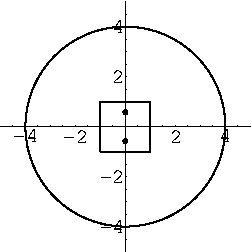
\includegraphics[width=0.25\textwidth]{fcv/cauchy/13z21}
      \end{center}
      \caption{The contours and the singularities.}
      \label{figure 13z21}
    \end{figure}
    We see that $C_1$ can be continuously deformed to $C_2$ on the domain where 
    the integrand is analytic.  Thus the integrals have the same value.
  \item 
    We consider the integrand
    \[
    \frac{z}{1 - \e^z}.
    \]
    Since $\e^z = 1$ has the solutions $z = \imath 2 \pi n$ for $n \in \mathbb{Z}$,
    the integrand has singularities at these points.
    There is a removable singularity at $z = 0$ and first order poles at 
    $z = \imath 2 \pi n$ for $n \in \mathbb{Z} \setminus \{ 0 \}$.
    Each contour contains only the singularity at $z = 0$. 
    See Figure~\ref{figure z1ez}.
    \begin{figure}[htb!]
      \begin{center}
        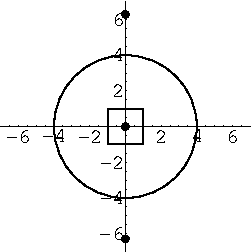
\includegraphics[width=0.25\textwidth]{fcv/cauchy/z1ez}
      \end{center}
      \caption{The contours and the singularities.}
      \label{figure z1ez}
    \end{figure}
    We see that $C_1$ can be continuously deformed to $C_2$ on the domain where 
    the integrand is analytic.  Thus the integrals have the same value.
  \end{enumerate}
\end{Solution}










\begin{Solution}
  First we write the integral of $f(z)$ as a sum of integrals.
  \begin{align*}
    \int_C f(z)\,\dd z
    &= \int_C \left( \frac{\alpha_k}{z^k} + \frac{\alpha_{k-1}}{z^{k-1}} + \cdots +\frac{\alpha_1}{z} + g(z) \right)
    \,\dd z
    \\
    &= \int_C \frac{\alpha_k}{z^k}\,\dd z + \int_C \frac{\alpha_{k-1}}{z^{k-1}}\,\dd z + \cdots 
    + \int_C \frac{\alpha_1}{z}\,\dd z + \int_C g(z)\,\dd z
  \end{align*}
  The integral of $g(z)$ vanishes by the Cauchy-Goursat theorem.  We evaluate 
  the integral of $\alpha_1 / z$ with Cauchy's integral formula.
  \[
  \int_C \frac{\alpha_1}{z}\,\dd z = \imath 2 \pi \alpha_1
  \]
  We evaluate the remaining $\alpha_n / z^n$ terms with anti-derivatives.  Each of 
  these integrals vanish.
  \begin{align*}
    \int_C f(z)\,\dd z
    &= \int_C \frac{\alpha_k}{z^k}\,\dd z + \int_C \frac{\alpha_{k-1}}{z^{k-1}}\,\dd z + \cdots 
    + \int_C \frac{\alpha_1}{z}\,\dd z + \int_C g(z)\,\dd z
    \\
    &= \left[ - \frac{\alpha_k}{(k - 1) z^{k - 1}} \right]_C 
    + \cdots + \left[ - \frac{\alpha_2}{z} \right]_C
    + \imath 2 \pi \alpha_1
    \\
    &= \imath 2 \pi \alpha_1
  \end{align*}  
\end{Solution}







\begin{Solution}
  We evaluate the integrals with the Cauchy integral formula.
  ($z_0$ is required to not be on $C$ so the integrals exist.)
  \begin{gather*}
    \int_C \frac{f'(z)}{z - z_0}\,\dd z 
    = \begin{cases}
      \imath 2 \pi f'(z_0) &\mathrm{if}\ z_0\ \mathrm{is inside}\ C
      \\
      0 &\mathrm{if}\ z_0\ \mathrm{is outside}\ C
    \end{cases}
    \\
    \int_C \frac{f(z)}{(z - z_0)^2}\,\dd z 
    = \begin{cases}
      \frac{\imath 2 \pi}{1!} f'(z_0) &\mathrm{if}\ z_0\ \mathrm{is inside}\ C
      \\
      0 &\mathrm{if}\ z_0\ \mathrm{is outside}\ C
    \end{cases}
  \end{gather*}
  Thus we see that the integrals are equal.
\end{Solution}









\begin{Solution}
  First we evaluate the integral using the Cauchy Integral Formula.
  \[
  \int_C \frac{\e^{a z}}{z} \,\dd z = \left[ \e^{a z} \right]_{z = 0} = \imath 2 \pi
  \]
  Next we parameterize the path of integration.  We use the periodicity
  of the cosine and sine to simplify the integral.
  \begin{gather*}
    \int_C \frac{\e^{a z}}{z} \,\dd z = \imath 2 \pi
    \\
    \int_0^{2 \pi} \frac{\e^{a \e^{\imath \theta}}}{\e^{\imath \theta}} \imath \e^{\imath \theta}\,\dd \theta = \imath 2 \pi
    \\
    \int_0^{2 \pi} \e^{a (\cos \theta + \imath \sin \theta)}\,\dd \theta = 2 \pi
    \\
    \int_0^{2 \pi} \e^{a \cos \theta} (\cos(\sin \theta) + \imath \sin(\sin \theta))\,\dd \theta = 2 \pi
    \\
    \int_0^{2 \pi} \e^{a \cos \theta} \cos(\sin \theta)\,\dd \theta = 2 \pi
    \\
    \int_0^\pi \e^{a \cos \theta} \cos(\sin \theta)\,\dd \theta = \pi
  \end{gather*}
\end{Solution}








\begin{Solution}
  \begin{enumerate}
    %%
  \item 
    We factor the integrand to see that there are singularities at 
    the cube roots of $9$.
    \[
    \frac{z}{z^3 - 9} = \frac{z}{\left( z - \sqrt[3]{9} \right)
      \left( z - \sqrt[3]{9} \e^{\imath 2 \pi/3} \right)
      \left( z - \sqrt[3]{9} \e^{-\imath 2 \pi/3} \right) }
    \]
    Let $C_1$, $C_2$ and $C_3$ be contours around $z = \sqrt[3]{9}$,
    $z = \sqrt[3]{9} \e^{\imath 2 \pi/3}$ and $z = \sqrt[3]{9} \e^{-\imath 2 \pi/3}$.  See 
    Figure~\ref{figure zz39}.  Let $D$ be the domain between $C$, $C_1$ and
    $C_2$, i.e. the boundary of $D$ is the union of $C$, $-C_1$ and $-C_2$.
    Since the integrand is analytic in $D$, the integral along the boundary
    of $D$ vanishes.
    \[
    \int_{\partial D} \frac{z}{z^3 - 9}\,\dd z
    = \int_{C} \frac{z}{z^3 - 9}\,\dd z
    + \int_{-C_1} \frac{z}{z^3 - 9}\,\dd z
    + \int_{-C_2} \frac{z}{z^3 - 9}\,\dd z
    + \int_{-C_3} \frac{z}{z^3 - 9}\,\dd z = 0
    \]
    From this we see that the integral along $C$ is equal to the sum of 
    the integrals along $C_1$, $C_2$ and $C_3$.  (We could also see this by deforming
    $C$ onto $C_1$, $C_2$ and $C_3$.)
    \[
    \int_{C} \frac{z}{z^3 - 9}\,\dd z = 
    \int_{C_1} \frac{z}{z^3 - 9}\,\dd z
    + \int_{C_2} \frac{z}{z^3 - 9}\,\dd z
    + \int_{C_3} \frac{z}{z^3 - 9}\,\dd z
    \]
    We use the Cauchy Integral Formula to evaluate the integrals along
    $C_1$, $C_2$ and $C_2$.
    \begin{align*}
      \int_C \frac{z}{z^3 - 9}\,\dd z
      &= \int_{C_1} \frac{z}{\left( z - \sqrt[3]{9} \right)
        \left( z - \sqrt[3]{9} \e^{\imath 2 \pi/3} \right)
        \left( z - \sqrt[3]{9} \e^{-\imath 2 \pi/3} \right) }\,\dd z
      \\
      &\quad + \int_{C_2} \frac{z}{\left( z - \sqrt[3]{9} \right)
        \left( z - \sqrt[3]{9} \e^{\imath 2 \pi/3} \right)
        \left( z - \sqrt[3]{9} \e^{-\imath 2 \pi/3} \right) }\,\dd z
      \\
      &\quad + \int_{C_3} \frac{z}{\left( z - \sqrt[3]{9} \right)
        \left( z - \sqrt[3]{9} \e^{\imath 2 \pi/3} \right)
        \left( z - \sqrt[3]{9} \e^{-\imath 2 \pi/3} \right) }\,\dd z
      \\
      &= \imath 2 \pi \left[ \frac{z}{
          \left( z - \sqrt[3]{9} \e^{\imath 2 \pi/3} \right)
          \left( z - \sqrt[3]{9} \e^{-\imath 2 \pi/3} \right) } \right]_{z = \sqrt[3]{9}}
      \\
      &\quad + \imath 2 \pi \left[ \frac{z}{
          \left( z - \sqrt[3]{9} \right)
          \left( z - \sqrt[3]{9} \e^{-\imath 2 \pi/3} \right) } 
      \right]_{z = \sqrt[3]{9} \e^{\imath 2 \pi/3}}
      \\
      &\quad + \imath 2 \pi \left[ \frac{z}{
          \left( z - \sqrt[3]{9} \right)
          \left( z - \sqrt[3]{9} \e^{\imath 2 \pi/3} \right) } 
      \right]_{z = \sqrt[3]{9} \e^{- \imath 2 \pi/3}}
      \\
      &= \imath 2 \pi 3^{-5/3} \left( 1 - \e^{\imath \pi/3} + \e^{\imath 2 \pi/3} \right)
      \\
      &= 0
    \end{align*}
    \begin{figure}[htb!]
      \begin{center}
        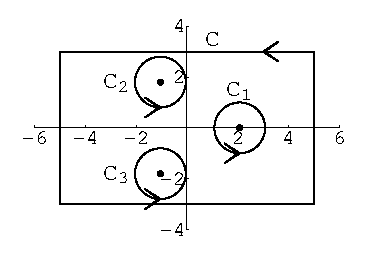
\includegraphics[width=0.4\textwidth]{fcv/cauchy/zz39}
      \end{center}
      \caption{The contours.}
      \label{figure zz39}
    \end{figure}
    %%
  \item 
    The integrand has singularities at $z = 0$ and $z = 4$.  Only the 
    singularity at $z = 0$ lies inside the contour.
    We use the Cauchy Integral Formula to evaluate the integral.
    \begin{align*}
      \int_C \frac{\sin z}{z^2 (z - 4)}\,\dd z
      &= \imath 2 \pi \left[ \frac{\dd}{\dd z} \frac{\sin z}{z - 4} \right]_{z = 0}
      \\
      &= \imath 2 \pi \left[ \frac{\cos z}{z - 4} - \frac{\sin z}{(z - 4)^2} \right]_{z = 0}
      \\
      &= - \frac{\imath \pi}{2}
    \end{align*}
    %%
  \item 
    We factor the integrand to see that there are singularities at $z = 0$ 
    and $z = - \imath$.
    \[
    \int_C \frac{(z^3 + z + \imath) \sin z}{z^4 + \imath z^3}\,\dd z
    = \int_C \frac{(z^3 + z + \imath) \sin z}{z^3 (z + \imath)}\,\dd z
    \]
    Let $C_1$ and $C_2$ be contours around $z = 0$ and $z = - \imath$.  See 
    Figure~\ref{figure z3zi-sinz-z4iz3}.
    Let $D$ be the domain between $C$, $C_1$ and
    $C_2$, i.e. the boundary of $D$ is the union of $C$, $-C_1$ and $-C_2$.
    Since the integrand is analytic in $D$, the integral along the boundary
    of $D$ vanishes.
    \[
    \int_{\partial D} = \int_{C} + \int_{-C_1} + \int_{-C_2} = 0
    \]
    From this we see that the integral along $C$ is equal to the sum of 
    the integrals along $C_1$ and $C_2$.  (We could also see this by deforming
    $C$ onto $C_1$ and $C_2$.)
    \[
    \int_{C} = \int_{C_1} + \int_{C_2}
    \]
    We use the Cauchy Integral Formula to evaluate the integrals along
    $C_1$ and $C_2$.
    \begin{align*}
      \int_C \frac{(z^3 + z + \imath) \sin z}{z^4 + \imath z^3}\,\dd z
      &= \int_{C_1} \frac{(z^3 + z + \imath) \sin z}{z^3 (z + \imath)}\,\dd z
      + \int_{C_2} \frac{(z^3 + z + \imath) \sin z}{z^3 (z + \imath)}\,\dd z
      \\
      &= \imath 2 \pi \left[ \frac{(z^3 + z + \imath) \sin z}{z^3} \right]_{z = -\imath}
      + \frac{\imath 2 \pi}{2!} \left[ \frac{\dd^2}{\dd z^2}
        \frac{(z^3 + z + \imath) \sin z}{z + \imath} \right]_{z = 0}
      \\
      &= \imath 2 \pi (- \imath \sinh(1))
      + \imath \pi \bigg[ 
      2 \left( \frac{3 z^2 + 1}{z + \imath} - \frac{z^3 + z + \imath}{(z + \imath)^2} 
      \right) \cos z 
      \\
      &\qquad + \left( \frac{6 z}{z + \imath} - \frac{2 (3 z^2 + 1)}{(z + \imath)^2}
        + \frac{2 (z^3 + z + \imath)}{(z + \imath)^3} 
        - \frac{z^3 + z + \imath}{z + \imath} \right) \sin z
      \bigg]_{z = 0}
      \\
      &= 2 \pi \sinh(1)
    \end{align*}
    \begin{figure}[htb!]
      \begin{center}
        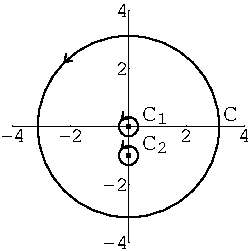
\includegraphics[width=0.3\textwidth]{fcv/cauchy/z3zi-sinz-z4iz3}
      \end{center}
      \caption{The contours.}
      \label{figure z3zi-sinz-z4iz3}
    \end{figure}
    %%
  \item 
    We consider the integral
    \[
    \int_C \frac{\e^{z t}}{z^2 (z + 1)}\,\dd z.
    \]
    There are singularities at $z = 0$ and $z = - 1$.
    \[
    \]
    Let $C_1$ and $C_2$ be contours around $z = 0$ and $z = - 1$.  See 
    Figure~\ref{figure ezt-z2z1}.  We deform $C$ onto $C_1$ and $C_2$.
    \[
    \int_{C} = \int_{C_1} + \int_{C_2}
    \]
    We use the Cauchy Integral Formula to evaluate the integrals along
    $C_1$ and $C_2$.
    \begin{align*}
      \int_C \frac{\e^{z t}}{z^2 (z + 1)}\,\dd z
      &= \int_{C_1} \frac{\e^{z t}}{z^2 (z + 1)}\,\dd z
      + \int_{C_1} \frac{\e^{z t}}{z^2 (z + 1)}\,\dd z
      \\
      &= \imath 2 \pi \left[ \frac{\e^{z t}}{z^2} \right]_{z = -1}
      + \imath 2 \pi \left[ \frac{\dd}{\dd z} \frac{\e^{z t}}{(z + 1)} \right]_{z = 0}
      \\
      &= \imath 2 \pi \e^{-t}
      + \imath 2 \pi \left[ \frac{t \e^{z t}}{(z + 1)} - \frac{\e^{z t}}{(z + 1)^2} 
      \right]_{z = 0}
      \\
      &= \imath 2 \pi (\e^{-t} + t - 1)
    \end{align*}
    \begin{figure}[htb!]
      \begin{center}
        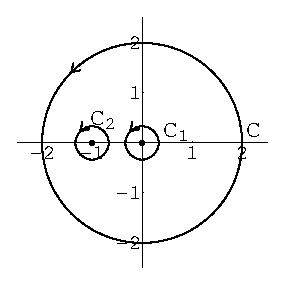
\includegraphics[width=0.25\textwidth]{fcv/cauchy/ezt-z2z1}
      \end{center}
      \caption{The contours.}
      \label{figure ezt-z2z1}
    \end{figure}
  \end{enumerate}
\end{Solution}







\begin{Solution}
  Liouville's Theorem states that if $f(z)$ is analytic and bounded 
  in the complex plane then $f(z)$ is a constant.
  \begin{enumerate}
  \item 
    Since $f(z)$ is analytic, $\e^{f(z)}$ is analytic.  The modulus of $\e^{f(z)}$
    is bounded.
    \[
    \left| \e^{f(z)} \right| = \e^{\Re(f(z))} \leq \e^M
    \]
    By Liouville's Theorem we conclude that $\e^{f(z)}$ is constant and hence
    $f(z)$ is constant.
  \item 
    We know that $f(z)$ is entire and $|f^{(5)}(z)|$ is bounded in the complex
    plane.  Since $f(z)$ is analytic, so is $f^{(5)}(z)$.  We apply Liouville's
    Theorem to $f^{(5)}(z)$ to conclude that it is a constant.  Then we integrate
    to determine the form of $f(z)$.
    \[
    f(z) = c_5 z^5 + c_4 z^4 + c_3 z^3 + c_2 z^2 + c_1 z + c_0
    \]
    Here $c_5$ is the value of $f^{(5)}(z)$ and $c_4$ through $c_0$ are constants of
    integration.
    We see that $f(z)$ is a polynomial of degree at most five.
  \end{enumerate}
\end{Solution}








\begin{Solution}
  For this problem we will use the 
  Extremum Modulus Theorem:
  Let $f(z)$ be analytic in a closed, connected domain, $D$.  The
  extreme values of the modulus of the function must occur on the
  boundary.  If $|f(z)|$ has an interior extrema, then the function
  is a constant.

  Since $|f(z)|$ has an interior extrema, $|f(0)| = |\e^\imath| = 1$, we conclude
  that $f(z)$ is a constant on $D$.  Since we know the value at $z = 0$,
  we know that $f(z) = \e^\imath$.
\end{Solution}







\begin{Solution}
  First we determine the radius of convergence of the series with the 
  ratio test.
  \begin{align*}
    R
    &= \lim_{k \to \infty} \left| \frac{ k^4 / 4^k }{ (k + 1)^4 / 4^{k + 1} } \right|
    \\
    &= 4 \lim_{k \to \infty} \frac{ k^4 }{ (k + 1)^4 }
    \\
    &= 4 \lim_{k \to \infty} \frac{ 24 }{ 24 }
    \\
    &= 4
  \end{align*}
  The series converges absolutely for $|z| < 4$.
  \begin{enumerate}
  \item 
    Since the integrand is analytic inside and on the contour of integration,
    the integral vanishes by Cauchy's Theorem.
  \item 
    \begin{align*}
      \int_C \frac{f(z)}{z^3}\,\dd z
      &= \int_C \sum_{k=0}^\infty k^4 \left( \frac{z}{4} \right)^k \frac{1}{z^3}\,\dd z
      \\
      &= \int_C \sum_{k=1}^\infty \frac{k^4}{4^k} z^{k-3}\,\dd z
      \\
      &= \int_C \sum_{k = -2}^\infty \frac{(k+3)^4}{4^{k + 3}} z^k\,\dd z
      \\
      &= \int_C \frac{1}{4 z^2}\,\dd z + \int_C \frac{1}{z}\,\dd z 
      + \int_C \sum_{k = 0}^\infty \frac{(k+3)^4}{4^{k + 3}} z^k\,\dd z
    \end{align*}
    We can parameterize the first integral to show that it vanishes.  The second
    integral has the value $\imath 2 \pi$ by the Cauchy-Goursat Theorem.  The third
    integral vanishes by Cauchy's Theorem as the integrand is analytic
    inside and on the contour.
    \[
    \int_C \frac{f(z)}{z^3}\,\dd z = \imath 2 \pi
    \]
  \end{enumerate}
\end{Solution}












\raggedbottom
}
